\documentclass[a4paper,11pt]{refart}

\usepackage[utf8]{inputenc}
\usepackage[T1]{fontenc}

\usepackage{textcomp}
\usepackage[lining,tabular]{fbb}

\usepackage{microtype}

\usepackage{graphicx}
\usepackage{enumitem}
\setlist{leftmargin=*}
\usepackage{listings}
\lstset{basicstyle=\ttfamily,frame=single,xleftmargin=3em,xrightmargin=3em}
\usepackage[os=win]{menukeys}
\renewmenumacro{\keys}[+]{shadowedroundedkeys}
\usepackage{framed}
\usepackage{etoolbox}
\AtBeginEnvironment{leftbar}{\sffamily\small}

\usetikzlibrary{chains,arrows,shapes,positioning}
\usepackage{hyperref}

\renewcommand\abstractname{Resumen}
\renewcommand{\contentsname}{Tabla de contenido}

\title{Lab. 03: Pre-procesamiento de señales sísmicas}
\author{David Duran (\url{davidamos.duran@unmsm.edu.pe})\\\url{https://totallynotdavid.github.io/}}
\date{\url{https://github.com/totallynotdavid/Teleseismic_Body-Wave_Inversion/}\\6 de noviembre, 2023}
\begin{document}
\maketitle

\begin{abstract}
    Este laboratorio está diseñado para estudiantes e investigadores interesados en el análisis de datos de ondas de cuerpo telesísmicas. Proporciona instrucciones detalladas sobre cómo utilizar un script de Python para automatizar la descarga, conversión y preparación de datos sísmicos. Utilizando el script, los usuarios pueden adquirir datos sísmicos en formato miniSEED y los metadatos correspondientes en formato XML. Posteriormente, se realiza la conversión a formatos SEED \footnote{SEED = Standard for Exchange of Earthquake Data} sin datos (dataless SEED) y a SAC mediante el uso de la herramienta `rdseed` \cite{rdseed}, la cual es esencial para el análisis subsecuente utilizando el modelo de Kikuchi y Kanamori \cite{kikuchi_kanamori_model}. Este proceso automatizado no solo mejora la eficiencia en el procesamiento de datos, sino que también asegura una mayor confiabilidad y estandarización en la manipulación de los mismos.
\end{abstract}

\tableofcontents
\clearpage

\section*{Flujo de trabajo del script}

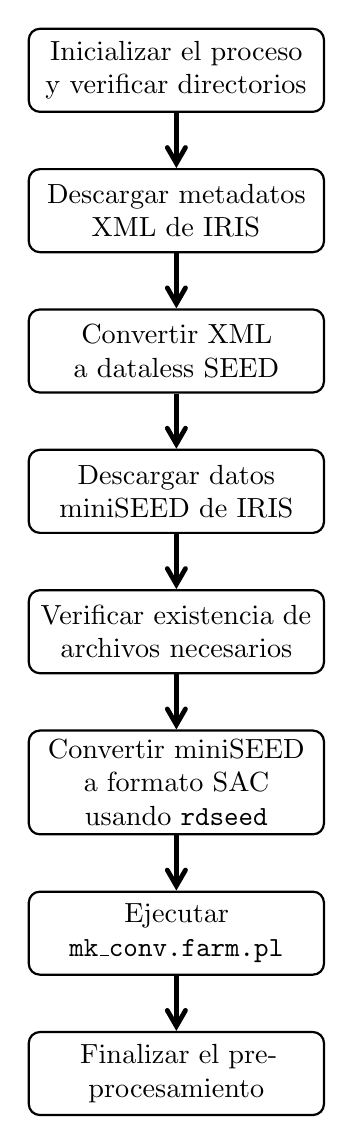
\begin{tikzpicture}
  \tikzset{
    every node/.style={
      on chain,
      draw,
      thick,
      rounded corners,
      minimum height=3em,
      text width=10em,
      align=center
    },
    line/.style={
      draw,
      thick,
      -latex',
      shorten >=2pt
    },
    every join/.style={line}
  }
  
  \begin{scope}[start chain=going below, node distance=0.7cm]
  \node (init) {Inicializar el proceso y verificar directorios};
  \node (downmeta) {Descargar metadatos XML de IRIS};
  \node (convertmeta) {Convertir XML a dataless SEED};
  \node (downseed) {Descargar datos miniSEED de IRIS};
  \node (convseed) {Verificar existencia de archivos necesarios};
  \node (seedtosac) {Convertir miniSEED a formato SAC usando \texttt{rdseed}};
  \node (postprocess) {Ejecutar \texttt{mk\_conv.farm.pl}};
  \node (end) {Finalizar el pre-procesamiento};
  \end{scope}

  \path[draw,line width=0.4ex, ->,>= angle 60]
  (init) edge (downmeta)
  (downmeta) edge (convertmeta)
  (convertmeta) edge (downseed)
  (downseed) edge (convseed)
  (convseed) edge (seedtosac)
  (seedtosac) edge (postprocess)
  (postprocess) edge (end);

\end{tikzpicture}

\section{Instalar dependencias}

Para realizar el análisis sísmico con el modelo de Kikuchi y Kanamori, es necesario instalar una serie de dependencias. A continuación, se presenta un resumen de los pasos que debes seguir para la instalación de estas herramientas esenciales.

\subsection{Herramientas necesarias}

Asegúrate de tener instaladas las siguientes herramientas:

\begin{itemize}
\item \textbf{rdseed}: Conversión de datos sísmicos a diversos formatos. Disponible para descarga en \url{http://www.iris.edu/pub/programs/rdseedv5.3.1.tar.gz}.
\item \textbf{Seismic Analysis Code} (SAC): Necesario para analizar y procesar datos sísmicos. El formulario de solicitud está disponible en \url{http://ds.iris.edu/ds/nodes/dmc/forms/sac/}.
\item \textbf{Java}: Requerido para ejecutar aplicaciones como el convertidor de StationXML a SEED. En Ubuntu puede instalarse con: \texttt{sudo apt install default-jre}
\item \textbf{Perl}: Usado para ejecutar scripts que manipulan archivos de datos sísmicos. En Ubuntu puede instalarse con: \texttt{sudo apt install perl}
\end{itemize}

\begin{leftbar}
  El proceso de instalación de estas herramientas puede variar dependiendo del sistema operativo que estés utilizando. Este proceso ha sido automatizado para Ubuntu (GNU Linux) en el archivo bash \texttt{dependencies.sh}. Para más información, consulta el archivo \texttt{README.md} en el repositorio de GitHub.
\end{leftbar}

\subsubsection{Pasos para la instalación}

Sigue estos pasos para configurar tu entorno de trabajo:

\begin{enumerate}
  \item Descarga o clona el repositorio que contiene todas las dependencias y scripts necesarios desde \url{https://github.com/totallynotdavid/Teleseismic_Body-Wave_Inversion/}.
  \begin{verbatim}
  git clone https://github.com/totallynotdavid/Teleseismic_Body-Wave_Inversion/
  \end{verbatim}
  \item Asegúrate de estar en la carpeta raíz del repositorio:
  \begin{verbatim}
  cd Teleseismic_Body-Wave_Inversion
  \end{verbatim}
  \item Otorga permisos de ejecución al script \texttt{dependencies.sh}:
  \begin{verbatim}
  chmod +x /scripts/bash/dependencies.sh
  \end{verbatim}
  \item Ejecuta el script para instalar todas las dependencias necesarias:
  \begin{verbatim}
  chmod /scripts/bash/dependencies.sh
  \end{verbatim}
\end{enumerate}

\section{Pre-procesamiento}

\subsection{Preparación de datos}

Antes de utilizar el modelo de Kikuchi y Kanamori, necesitas preparar tus datos en el formato SAC \footnote{SAC headers contienen información sobre la inclinación y el azimut.}. Para ello, utiliza el siguiente script de Python, el cual automatiza la descarga y el procesamiento inicial de los datos sismicos.

\begin{enumerate}
\item Ejecuta el script con Python:
\begin{verbatim}
python3 /scripts/python/fetch_and_process.py
\end{verbatim}
El script procederá con la descarga y conversión de datos, preparándolos para el análisis con el modelo.
\item Para eliminar archivos innecesarios y mantener el orden, utiliza el script de limpieza proporcionado:
\begin{verbatim}
chmod +x /scripts/bash/cleaning.sh
./scripts/bash/cleaning.sh
\end{verbatim}

\end{enumerate}

\subsection{Procesamiento final con Perl}

Finalmente, para convertir los datos al formato deseado por el modelo:
  \begin{enumerate}
  \item Navega a la carpeta de scripts de Perl y copia el script necesario a la carpeta de datos:
  \begin{verbatim}
  cp mk_conv.farm.pl /data/preprocesamiento/
  cd /data/preprocesamiento/
  \end{verbatim}
  \item Ejecuta el script de Perl para completar la conversión:
  \begin{verbatim}
  perl mk_conv.farm.pl
  \end{verbatim}
\end{enumerate}
Con estos pasos, tendrás los datos listos para ser utilizados en el pipeline del modelo de Kikuchi y Kanamori.

\section{Detalles técnicos}

El proceso de procesamiento de señales sísmicas se apoya en una serie de scripts diseñados para automatizar las tareas que van desde la adquisición de los datos hasta su preparación definitiva para el análisis correspondiente con el modelo. A continuación, se delinean los componentes técnicos fundamentales de la fase inicial del flujo de trabajo, establecido por el autor. Esta fase se maneja de forma independiente al modelo de Kikuchi y Kanamori.

\subsection{Descarga de datos}

Para la automatización de los requests con la base de datos de SAGE (\textit{Seismological Facility for the Advancement of Geoscience}), se ha desarrollado el script \texttt{fetch\_and\_process.py}. Este script está concebido para facilitar la recolección eficiente de los datos sísmicos junto con sus respectivos metadatos. Es necesario, claro está, definir las estaciones apropiadas y los rangos de tiempo apropiados para el investigador.

En el pasado, la adquisición de archivos en formato SAC se realizaba automáticamente a través del portal Wilber 3; sin embargo, dicha funcionalidad fue descontinuada en el 2021 en favor de los archivos miniSEED. A raíz de esto, es ahora requisito construir el archivo SAC manualmente, utilizando los datos obtenidos en formato miniSEED, complementándolos con los metadatos en el formato dataless y los polos y ceros necesarios.

\begin{itemize}
    \item \textbf{Metadatos:} El servicio web FDSN se emplea para obtener metadatos en formato XML, que ofrecen información detallada sobre las estaciones sísmicas, incluyendo sus ubicaciones, equipamiento y características de las señales registradas. Estos metadatos son cruciales para la interpretación correcta de los datos sísmicos.
    \item \textbf{Datos Sísmicos:} Se descargan los registros sísmicos en formato miniSEED. Este formato es la elección estándar en la industria para el almacenamiento y transmisión de datos sísmicos debido a su eficiencia y amplia adopción, lo que asegura compatibilidad y facilidad de uso en diversas aplicaciones de análisis.
\end{itemize}

El script está configurado para procesar datos de múltiples estaciones sísmicas.

\subsection{Verificación de archivos necesarios}

Antes de proceder con la conversión de miniSEED a SAC, el script realiza una verificación para asegurarse de que todos los archivos necesarios estén presentes. Esto incluye la presencia de los archivos dataless y los archivos miniSEED. Si falta algún archivo, el script alertará al usuario y detendrá el proceso para evitar errores en el procesamiento posterior.

\subsection{Uso de \texttt{rdseed}}

Para la conversión de miniSEED a SAC, se emplea el programa \texttt{rdseed}. Es una herramienta que permite la extracción de datos de archivos SEED (incluyendo miniSEED y dataless SEED) y su conversión a otros formatos, en este caso, al formato SAC utilizado ampliamente en el análisis sísmico.

\subsection{Scripts Perl para Procesamiento Final}

\texttt{mk\_conv.farm.pl} (brindado por Kikuchi y Kanamori en el manual de su modelo) es utilizado en la etapa final del pre-procesamiento para automatizar el procesamiento de grandes conjuntos de datos. Este script generará dos archivos: \texttt{response} y \texttt{i\_conv.farm}.

\subsection{Entorno de ejecución}

El entorno de ejecución para los scripts está configurado para ser lo más automatizado posible, reduciendo la necesidad de intervención manual y permitiendo que los investigadores se centren en el análisis de los datos en lugar de en su preparación.

\begin{itemize}
\item Se asume que las dependencias y el entorno (Fortran77, Java, Perl) han sido instalados y configurados adecuadamente, según se describe en las secciones previas de la guía.
\item Se espera que el sistema operativo sea compatible con los scripts de Bash y Python, así como con las herramientas Fortran y Perl.
\end{itemize}

\subsection{Documentación y soporte}

El código de cada script está ampliamente documentado internamente para facilitar la comprensión de su funcionamiento y la personalización de los procesos. Para problemas complejos o consultas específicas, se recomienda contactar al autor del script. El correo se encuentra en la portada de este documento.

\bibliographystyle{plain}
\bibliography{refs}
\end{document}